\documentclass{article}[11pt]
\setcounter{secnumdepth}{5}
\setcounter{tocdepth}{5}
\usepackage[english]{babel}
\usepackage{textcomp}
\usepackage{amsmath,amsthm,amsfonts,amssymb,epsfig}
\usepackage{array}
\usepackage{datetime}
\usepackage{lipsum}% http://ctan.org/pkg/lipsum
\usepackage[left=1.1in,top=1in,right=1.1in]{geometry}% http://ctan.org/pkg/geometry
\usepackage{listings}% http://ctan.org/pkg/listings
\usepackage{spverbatim}
\usepackage{hyperref}
\usepackage{microtype}
\hypersetup{colorlinks=true, urlcolor=black, linkcolor=black}
\usepackage{graphicx}
\graphicspath{ {images/} }
\usepackage{parskip}
\usepackage{titlesec} %used for diminishing heading sizes

\titleformat*{\section}{\LARGE\bfseries\sffamily}
\titleformat*{\subsection}{\Large\bfseries\sffamily}
\titleformat*{\subsubsection}{\large\bfseries\sffamily}
\titleformat*{\paragraph}{\large\bfseries\sffamily}
\titleformat*{\subparagraph}{\large\bfseries\sffamily}
\renewcommand{\familydefault}{\sfdefault} %sans-serif font

\begin{document}

\thispagestyle{empty} %removes page number  

\begin{center}
\textsc{\Large\bf{Gradient Boosted Machines with H2O's R Package}}
\\
\bigskip
\textsc{\small{Cliff Click \hspace{40pt} Michal Malohlava \hspace{40pt} Viraj Parmar \hspace{40pt} Jessica Lanford}}
\\
\bigskip
\line(1,0){250}  %inserts  horizontal line

\bigskip
August 2015: Third Edition 
\\%add front page image here? (wavy lines)
\bigskip
\end{center}

{\raggedright\vfill\ 

Gradient Boosted Machines with H2O's R Package\\
  by Cliff Click, Michal Malohlava, Viraj Parmar, \&\ Jessica Lanford\\
\bigskip
  Published by H2O.ai, Inc. \\
2307 Leghorn St. \\
Mountain View, CA 94043\\
\bigskip
\textcopyright 2015 H2O.ai, Inc. All Rights Reserved. 
\bigskip

August 2015: Third Edition
\bigskip

Photos by \textcopyright H2O.ai, Inc. 
\bigskip

While every precaution has been taken in the\\
preparation of this book, the publisher and\\
authors assume no responsibility for errors or\\
omissions, or for damages resulting from the\\
use of the information contained herein.\\
\bigskip
Printed in the United States of America. 


}\par

\newpage
\tableofcontents

\newpage
\section{What is H2O?}

H2O is fast scalable open-source machine learning and deep learning for Smarter Applications. With H2O, enterprises like PayPal, Nielsen, Cisco and others can use all of their data without sampling and get accurate predictions faster. Advanced algorithms, like Deep Learning, Boosting and Bagging Ensembles are readily available for application designers to build smarter applications through elegant APIs. Some of our earliest customers have built powerful domain-specific predictive engines for Recommendations, Customer Churn, Propensity to Buy, Dynamic Pricing and Fraud Detection for the Insurance, Healthcare, Telecommunications, AdTech,
Retail and Payment Systems.

Using in-memory compression techniques, H2O can handle billions of data rows in-memory, even with a fairly small cluster. The platform includes interfaces for R, Python, Scala, Java, JSON and Coffeescript/JavaScript, along with a built-in  web interface, Flow, that make it easier for non-engineers to stitch together complete analytic workflows. The platform was built alongside (and on top of) both Hadoop and Spark Clusters and is typically deployed within minutes.

H2O implements almost all common machine learning algorithms, such as generalized linear modeling (linear regression, logistic regression, etc.), Na\"{i}ve Bayes, principal components analysis, time series, k-means clustering and others. H2O also implements best-in-class algorithms such as Random Forest, Gradient Boosting and Deep Learning at scale. Customers can build thousands of models and compare them to get the best prediction results.

H2O is nurturing a grassroots movement of physicists, mathematicians, computer and data scientists to herald the new wave of discovery with data science. Academic researchers and Industrial data scientists collaborate closely with our team to make this possible. Stanford university giants Stephen Boyd, Trevor Hastie, Rob Tibshirani advise the H2O team to build scalable machine learning algorithms. With 100s of meetups over the past two years, H2O has become a word-of-mouth phenomenon growing amongst the data community by a 100-fold and is now used by 12,000+ users, deployed in 2000+ corporations using R, Python, Hadoop and Spark.

\textbf{Try it out}

H2O offers an R package that can be installed from CRAN. H2O can be downloaded at {\url{www.h2o.ai/download}}.

\textbf{Join the community}

Connect with {\url{h2ostream@googlegroups.com}} and {\url{https://github.com/h2oai}} to learn about our meetups, training sessions, hackathons, and product updates.

\textbf{Learn more about H2O}

Visit {\url{www.h2o.ai}}.

\section{Introduction}

This vignette presents the gradient boosted machine (GBM) framework in the H2O package at {\url{http://cran.r-project.org/web/packages/h2o/index.html}}. Further documentation on H2O's system and algorithms can be found at the h2o.ai website at {\url{http://docs.h2o.ai}} and the R package manual at {\url{http://cran.r-project.org/web/packages/h2o/h2o.pdf}}. The full datasets and code of this vignette can be found at the H2O Github at {\url{http://github.com/h2oai/h2o}}. This introductory section provides instructions on getting H2O started, followed by a brief overview of gradient boosting.


\section{Installation}

To use H2O with R, you can start H2O outside of R and connect to it, or you can launch H2O from R. However, if you launch H2O from R and close the R session, the H2O instance is closed as well. The client object is used to direct R to datasets and models located in H2O.

\subsection{Installing R or R Studio}

To download R:
\begin{enumerate}
\item Go to {\url{http://cran.r-project.org/mirrors.html}}. 
\item Select your closest local mirror. 
\item Select your operating system (Linux, OS X, or Windows). 
\item Depending on your OS, download the appropriate file, along with any required packages. 
\item When the download is complete, unzip the file and install. \\
\end{enumerate}

To download R Studio: 

\begin{enumerate}
\item Go to {\url{http://www.rstudio.com/products/rstudio/}}. 
\item Select your deployment type (desktop or server). 
\item Download the file. 
\item When the download is complete, unzip the file and install.
\end{enumerate}


\subsection{Installing H2O in R}
\begin{enumerate}
\item Load the latest CRAN H2O package by running \begin{spverbatim} install.packages("h2o") \end{spverbatim}\footnote{Note: Our push to CRAN will be behind the bleeding edge version and due to resource constraints, may be behind the published version. However, there is a best-effort to keep the versions the same.} 

\footnotesize %need so that code fits on 1 line - using this instead of {lstlisting} since it looks better
\begin{spverbatim}
# The following two commands remove any previously installed H2O packages for R.
if ("package:h2o" %in% search()) { detach("package:h2o", unload=TRUE) }
if ("h2o" %in% rownames(installed.packages())) { remove.packages("h2o") }

# Next, we download packages that H2O depends on.
if (! ("methods" %in% rownames(installed.packages()))) { install.packages("methods") }
if (! ("statmod" %in% rownames(installed.packages()))) { install.packages("statmod") }
if (! ("stats" %in% rownames(installed.packages()))) { install.packages("stats") }
if (! ("graphics" %in% rownames(installed.packages()))) { install.packages("graphics") }
if (! ("RCurl" %in% rownames(installed.packages()))) { install.packages("RCurl") }
if (! ("rjson" %in% rownames(installed.packages()))) { install.packages("rjson") }
if (! ("tools" %in% rownames(installed.packages()))) { install.packages("tools") }
if (! ("utils" %in% rownames(installed.packages()))) { install.packages("utils") }
\end{spverbatim}
\begin{spverbatim}
# Now we download, install and initialize the H2O package for R (replacing
the * with the latest version number obtained from the H2O download page)
install.packages("h2o", type="source", repos=(c("http://h2o-release.s3.amazonaws.com/h2o/master/*/R")))
library(h2o)
localH2O = h2o.init(nthreads = -1)
\end{spverbatim}
\normalsize%restore default text size
To see {\texttt{h2o.gbm}} at work, run the following command to observe an automatic demo of an example classification model built using H2O's GBM.

\begin{spverbatim}
demo(h2o.gbm)
\end{spverbatim}
\end{enumerate}

\subsection{Making a build from Source Code}

If you are a developer who wants to make changes to the R package before building and installing it, pull the source code from Git (\url{https://github.com/h2oai/h2o}) and follow the instructions in From Source Code (Github) at {\url{http://docs.h2o.ai/developuser/quickstart\_git.html}}.

After making the build, navigate to the Rcran folder with the R package in the build’s directory, then run and install.
\begin{spverbatim}
 cd ~/Documents/h2o/target/Rcran (master)
$ R CMD INSTALL h2o_version#.tar.gz
* installing to library 'C:/Users/H2O-User/Documents/R/win-library/3.0'
* installing *source* package 'h2o' ...
** R
** demo
** inst
** preparing package for lazy loading
Warning: package 'statmod' was built under R version 3.0.3
Creating a generic function for 'summary' from package 'base' in package 'h2o'
Creating a generic function for 'colnames' from package 'base' in package 'h2o'
Creating a generic function for 't' from package 'base' in package 'h2o'
Creating a generic function for 'colnames<-' from package 'base' in package 'h2o'
Creating a generic function for 'nrow' from package 'base' in package 'h2o'
Creating a generic function for 'ncol' from package 'base' in package 'h2o'
Creating a generic function for 'sd' from package 'stats' in package 'h2o'
Creating a generic function for 'var' from package 'stats' in package 'h2o'
Creating a generic function for 'as.factor' from package 'base' in package 'h2o'
Creating a generic function for 'is.factor' from package 'base' in package 'h2o'
Creating a generic function for 'levels' from package 'base' in package 'h2o'
Creating a generic function for 'apply' from package 'base' in package 'h2o'
Creating a generic function for 'findInterval' from package 'base' in package 'h2o'
** help
*** installing help indices
** building package indices
** testing if installed package can be loaded
*** arch - i386
Warning: package 'statmod' was built under R version 3.0.3
*** arch - x64
Warning: package 'statmod' was built under R version 3.0.3
* DONE (h2o)
\end{spverbatim}


\section{H2O Initialization}

Use the command {\texttt{h2o.init()}} to launch H2O. The following section describes the parameters for the {\texttt{h2o.init()}} command. 

\subsection{H2O Initialization Parameters}

The {\texttt{h2o.init()}} command creates an H2O cluster or establishes a connection to an existing cluster. The following parameters are supported: 

\begin{itemize}
\item {\texttt{ip}}: Specify an IP address for H2O
\item {\texttt{port}}: Specify a port for H2O
\item {\texttt{startH2O}}: Enable ({\texttt{startH2O = TRUE}}) or disable ({\texttt{startH2O = FALSE}}) H2O initialization from R if no connection with H2O is detected. This option is enabled only is {\texttt{ip = "localhost"}} or {\texttt{ip = "127.0.0.1"}}. If an existing connection is detected, R does not initialize H2O. 
\item {\texttt{forceDL}}: Enable ({\texttt{forceDL = TRUE}}) or disable ({\texttt{forceDL = FALSE}}) forced downloads of the H2O executable. The default value is {\texttt{FALSE}}, so the executable is  only downloaded if it does not already exist in the H2O R library resources directory, {\texttt{h2o/java/h2o.jar}}. This option is only enabled when H2O is started from R. 
\item {\texttt{beta}}:  Enable ({\texttt{beta = TRUE}}) or disable ({\texttt{beta = FALSE}}) beta mode. 
\item {\texttt{assertion}}: Launch H2O with ({\texttt{assertion = TRUE}}) or without ({\texttt{assertion = FALSE}}) assertions. Use this mode for error checking and debugging. 
\item {\texttt{license}}: Specify the full path of the license file to enable additional features. 
\item {\texttt{nthreads}}: Specify the number of threads in the thread pool, which is related to the number of CPUs used. To use the CRAN default (2 CPUs), enter {\texttt{-2}}. To use all CPUs on the host, enter {\texttt{-1}}. To specify the number of CPUs, enter a positive integer. 
\item {\texttt{max\_mem\_size}}: Specify the maximum amount (in bytes) of memory to allocate to H2O. The value must be greater than 2MB and a multiple of 1024. Enter {\texttt{m}} or {\texttt{M}} to specify megabytes or enter {\texttt{g}} or {\texttt{G}} to specify gigabytes. 
\item {\texttt{min\_mem\_size}}: Specify the minimum amount (in bytes) of memory to allocate to H2O. Specify the maximum amount (in bytes) of memory to allocate to H2O. The value must be greater than 2MB and a multiple of 1024. Enter {\texttt{m}} or {\texttt{M}} to specify megabytes or enter {\texttt{g}} or {\texttt{G}} to specify gigabytes.
\end{itemize}


\subsection{Launching from R}

If you do not specify the argument {\texttt{max\_mem\_size}} when you run {\texttt{h2o.init( )}}, the default heap size of the H2O instance running on 32-bit Java is 1g. H2O checks the Java version and suggests an upgrade if you are running 32-bit Java. On 64-bit Java, the heap size is 1/4 of the total memory available on the machine. 

For best performance, the allocated memory should be 4x the size of your data, but never more than the total amount of memory on your computer. For larger data sets, we recommend running on a server or service with more memory available for computing.


To launch H2O from R, run the following in R:
\begin{spverbatim}
> library(h2o) # # Loads required files for H2O
localH2O <- h2o.init(ip = 'localhost', port = 54321, nthreads= -1, max_mem_size = ‘4g') # # Starts H2O on the localhost, port 54321, with 4g of memory using all CPUs on the host  \end{spverbatim} 
\\

R displays the following output: 
\begin{spverbatim}
Successfully connected to http://localhost:54321
       R is connected to H2O cluster:
   H2O cluster uptime:         11 minutes 35 seconds
   H2O cluster version:        2.7.0.1497
   H2O cluster name:           H2O_started_from_R
   H2O cluster total nodes:    1
   H2O cluster total memory:   3.56 GB
   H2O cluster total cores:    8
   H2O cluster allowed cores:  8
   H2O cluster healthy:        TRUE
\end{spverbatim}

If you are operating on a single node, initialize H2O using \begin{spverbatim} h2o_server = h2o.init()\end{spverbatim}\\

To connect with an existing H2O cluster node other than the default localhost:54321, specify the IP address and port number in the parentheses. For example:
\begin{spverbatim}h2o_cluster = h2o.init(ip = "192.555.1.123", port = 12345)\end{spverbatim}


\subsection{Launching from the Command Line}

After launching the H2O instance, initialize the connection by running {\texttt{h2o.init( )}} with the IP address and port number of a node in the cluster. In the following example, change 192.168.1.161 to your local host. 
\begin{spverbatim}
> library(h2o)
> localH2O <- h2o.init(ip = '192.168.1.161', port =54321)
\end{spverbatim}

\subsection{Launching on Hadoop}

To launch H2O nodes and form a cluster on the Hadoop cluster, run:

\begin{lstlisting}[breaklines,basicstyle=\ttfamily]

hadoop jar h2odriver_hdp2.1.jar water.hadoop.h2odriver -libjars ../h2o.jar -mapperXmx 1g -nodes 1 -output hdfsOutputDirName

\end{lstlisting}

\begin{itemize}
\item For each major release of each distribution of Hadoop, there is a driver jar file that the user will need to launch H2O with. Currently available driver jar files in each build of H2O include {\texttt{h2odriver_cdh5.jar, h2odriver_hdp2.1.jar}}, and {\texttt{mapr2.1.3.jar}}.
\item The above command launches exactly one 1g node of H2O; however,  we recommend launching the cluster with 4 times the memory of your data file.
\item{\texttt{mapperXmx}} is the mapper size or the amount of memory allocated to each node.
\item{\texttt{nodes}} is the number of nodes requested to form the cluster.
\item{\texttt{output}} is the name of the directory created each time a H2O cloud is created so it is necessary for the name to be unique each time it is launched.
\end{itemize}


\subsection{Launching on an EC2}

Launch the EC2 instances using the H2O AMI by running {\texttt{h2o-cluster-launch-instances.py}.

\begin{spverbatim}
$ python h2o-cluster-launch-instances.py
Using boto version 2.27.0
Launching 2 instances.
Waiting for instance 1 of 2 ...
  .
  .
  instance 1 of 2 is up.
Waiting for instance 2 of 2 ...
  instance 2 of 2 is up.

\end{spverbatim}

\subsection{Checking Cluster Status}


To check the status and health of the H2O cluster, use {\texttt{h2o.clusterInfo( )}}.
\begin{spverbatim}
> library(h2o)
> localH2O = h2o.init(ip = 'localhost', port = 54321)
> h2o.clusterInfo(localH2O)
\end{spverbatim}

An easy-to-read summary of information about the cluster displays. 
\begin{spverbatim}
R is connected to H2O cluster:
  H2O cluster uptime:         43 minutes 43 seconds
  H2O cluster version:        2.7.0.1497
  H2O cluster name:           H2O_started_from_R
  H2O cluster total nodes:    1
  H2O cluster total memory:   3.56 GB
  H2O cluster total cores:    8
  H2O cluster allowed cores:  8
  H2O cluster healthy:        TRUE
\end{spverbatim}

\noindent

\subsection{Support} 
Users of the H2O package may submit general enquiries and bug reports to h2o.ai support at {\url{h2ostream@googlegroups.com}}. Alternatively, specific bugs or issues may be filed to the h2o.ai JIRA at {\url{https://0xdata.atlassian.net/secure/Dashboard.jspa}}.

\subsection{Gradient Boosting Overview} 

A gradient boosted model is an ensemble of tree models that can be either regression or classification. Both are forward-learning ensemble methods that obtain predictive results through gradually improved estimations. Boosting is a flexible nonlinear regression procedure that helps improve the accuracy of trees. By sequentially applying weak classification algorithms to the incrementally changed data, a series of decision trees are created that produce an ensemble of weak prediction models.

While boosting trees increases their accuracy, it also decreases speed and interpretability. The gradient boosting method generalizes tree boosting to minimize these issues. 

\subsubsection{Summary of features} 
H2O's GBM functionalities include:

\begin{itemize}

\item supervised learning for regression and classification tasks

\item distributed and parallelized computation on either a single node or a multi-node cluster

\item fast and memory-efficient Java implementations of the underlying algorithms

\item user-friendly web interface to mirror the model building and scoring process running in R

\item grid search for hyperparameter optimization and model selection

\item model export in plain Java code for deployment in production environments

\item additional parameters for model tuning

\end{itemize}

\subsubsection{Common Model Parameters}

This section describes the functions of the parameters for GBM: 

\begin{itemize}

\item {\texttt{x}}: The names or indices of the predictor variables for use in building the gradient boosted model. 

\item {\texttt{y}}: The name or index of the response variable (must be an integer or a categorical variable). If the data does not contain a header, {\texttt{y}} is the column index number starting at 0 and increasing from left to right. 

\item {\texttt{key}}: The unique hex key assigned to the generated model. If left blank, a key is automatically generated. 

\item \texttt{loss}: Enter {\texttt{AUTO}} or {\texttt{Bernoulli}} to select the loss type. The default is {\texttt{AUTO}}. 

\item {\texttt{ntrees}}: A non-negative integer that defines the number of trees. The default is 50. 

\item {\texttt{max\_depth}}: The user-defined tree depth. The default is 5. 

\item {\texttt{min\_rows}}: The minimum number of rows to assign to the terminal nodes. The default is 10. 

\item {\texttt{learn\_rate}}:An integer that defines the learning rate. The default is 0.1 and the range is 0.0 to 1.0. 

\item {\texttt{nbins}}: The number of bins to use for building the histogram. The default is 20. 

\item {\texttt{validation\_frame}}: An {\texttt{H2OFrame}} object that defines the validation dataset used to construct the confusion matrix. If left blank and {\texttt{nfolds = 0}}, the default is the training dataset.

\item {\texttt{balance\_classes}}: Balance training data class counts via over or undersampling for imbalanced data. The default is {\texttt{FALSE}}. 

\item {\texttt{max\_after\_balance\_size}}: Maximum relative size of the training data after balancing class counts; can be less than 1.0.  The default is 1. 

\item {\texttt{seed}}: Seed for random numbers that affects sampling. 

\item {\texttt{data}}: An {\texttt{H2OFrame}} object that contains the variables in the model. 

\item {\texttt{nfolds}}: Number of folds for cross-validation. If {\texttt{nfolds >= 2}}, then {\texttt{validation}} must be blank. 

\end{itemize}

\subsubsection{Theory and framework} 

Gradient boosting is a machine learning technique that combines two powerful tools: gradient-based optimization and boosting. Gradient-based optimization uses gradient computations to minimize a model's loss function with respect to the training data. Boosting additively collects an ensemble of weak models in order to ultimately create a strong learning system for predictive tasks. Here we consider gradient boosting in the example of K-class classification, although the model for regression follows similar logic. The following analysis follows from the discussion in Hastie et al (2010) at {\url{http://statweb.stanford.edu/~tibs/ElemStatLearn/}}.
\newline
\\
{\bf{\footnotesize{GBM for classification}}}
\\
\line(1,0){500}
\\ 
1. Initialize $f_{k0} = 0, k = 1,2,\dots,K$ 
\\
2. For $m=1$ to $M$
\\
\indent a. Set $p_k(x) = \frac{e^{f_k(x)}}{\sum_{l=1}^K e^{f_l(x)}}$ for all $k = 1,2\dots, K$
\\
\indent b. For $k=1$ to $K$
\\
\indent \indent i. Compute $r_{ikm} = y_{ik} - p_k(x_i),  i = 1,2,\dots,N$
\\
\indent \indent ii. Fit a regression tree to the targets $r_{ikm}, i = 1,2,\dots,N$, 
\par \hspace{3em} giving terminal regions $R_{jkm}, 1,2,\dots,J_m$
\\
\indent \indent iii. Compute $$\gamma_{jkm} = \frac{K-1}{K} \frac{\sum_{x_i \in R_{jkm}} (r_{ikm})}{\sum_{x_i \in R_{jkm}} |r_{ikm}| (1 - |r_{ikm}|)} , j=1,2,\dots,J_m$$
\\
\indent \indent iv. Update $f_{km}(x) = f_{k,m-1}(x) + \sum_{j=1}^{J_m} \gamma_{jkm} I(x \in R_{jkm})$
\\
3. Output $f_k^{\hat{}}(x) = f_{kM}(x),  k=1,2,\dots,K$
\\
\line(1,0){500}
\\
\\ 
In the above algorithm, for $k$-classification, H2O builds $k$-regression trees to represent one classification tree. The index $m$ tracks of the number of weak learners added to the current ensemble. Within this outer loop, there is an inner loop across each of the $K$ classes. In this inner loop, the first step is to compute the residuals, $r_{ikm}$, which are actually the gradient values, for each of the $N$ bins in the CART model, and then to fit a regression tree to these gradient computations. This fitting process is distributed and parallelized, and details on this framework can be found on the h2o.ai blog at {\url{http://h2o.ai/blog/2013/10/building-distributed-gbm-h2o/}}.
\\
\\
The final procedure in the inner loop is to add to the current model to the fitted regression tree, which improves the accuracy of the model during the inherent gradient descent step. After $M$ iterations, the final ``boosted" model can be tested out on new data.

\subsubsection{Loss Function}

The AdaBoost method builds an additive logistic regression model:

$${F(x) = log}\frac{Pr(Y = 1|x)}{Pr(Y = -1|x)} = \sum_{m=1}^{M} \alpha_m f_m (x) $$

by stagewise fitting using the loss function: 

$$L(y, F(x)) = exp(-y  F (x)) $$



\subsubsection{Distributed Trees}

In H2O's implementation of GBM, distributed trees are used. H2O overlays trees on the data by assigning a tree node to each row. The nodes are numbered and the number of each node is stored in a temporary vector as "Node\_ID" for each row. H2O makes a pass over all the rows using the most efficient method, which is not necessarily numerical order. A local histogram using local data only is created in parallel for each row on each node. The histograms are then assembled and a split column is selected to make the decision. The rows are re-assigned to nodes and the entire process is repeated. 

For example, for an initial tree, all rows start on node 0. A MapReduce (MR) task computes the statistics and uses them to make an algorithmically-based decision, such as lowest mean squared error (MSE). In the next layer in the tree (and the next MR task), a decision is made for each row: if X $<$ 1.5, go right in the tree; otherwise, go left. H2O computes the stats for each new leaf in the tree, and each pass across all the rows builds the entire layer. 

For multinomial or binomial, the split is determined by the number of columns. The number of columns is evaluated to find the best split out of the possible combinations. For example, for a hundred-column dataset that uses twenty bins, there are 2000 (20x100) possible split points. 

Each layer represents another MR task; therefore, a tree that is five layers deep requires five passes. Each tree level is fully data-parallelized. Each pass is over one layer in the tree, and builds a per-node histogram in the MR calls. As each pass analyzes a tree level, H2O then decides how to build the next level. H2O reassigns rows to new levels in another pass by merging the two passes and builds a histogram for each node. Each per-level histogram is done in parallel. 

Scoring and building is done in one pass. Each row is tested against the decision from the previous pass, assigned to a new leaf, and a histogram is built on that leaf. To score, H2O traverses the tree and obtains the results. The tree is compressed to a smaller object that can still be traversed, scored, and printed. 

Although the GBM algorithm builds each tree one level at a time, H2O is able to quickly run the entire level in parallel and distributed. More data can be offset by more CPUs or nodes.  Since H2O does the per-level compute in parallel, which requires sending histograms over the network, the amount of data can become very large for a very deep tree. 

High max-bin sizes slow down generation of deep trees, but this is not an issue for GBM tree depths, as GBM typically uses very shallow trees. Bin limits over 20 have been shown to have very little improvement on the quality of the GBM model. 

For the MSE reports, the zero-tree report uses the class distribution as the prediction. The one-tree report actually uses the first tree, so the first two reports are not equal. The reported MSE is the inclusive effect of all prior trees, and generally decreases monotonically on the training dataset. However, the curve will generally bottom out and then begin to slowly rise on the validation set as overfitting sets in. 

The computing cost is based on the number of leaves, but depending on the dataset, the number of leaves can be difficult to predict. The maximum number of leaves is $2^d$, where $d$ represents the tree depth.

\subsubsection{Treatment of factors}

When the specified GBM model includes factors, those factors are analyzed by assigning an integer to each distinct factor level, and then binning the ordered integers according to the user-specified number of bins ($N$ bins). Split points are determined by considering the end points of each bin and the one-versus-many split for each bin. 

For example, if the factor is split into five bins, H2O orders the bins by bin number, then considers the split between the first and second bin, then the second and third, then the third and fourth, and the fourth and fifth. Additionally, the split that results from splitting the first bin from the other four and all analogous splits for the other four bins are considered. To specify a model that considers all factors individually, set the value for $N$ bins equal to the number of factor levels. This can be done for over 1024 levels (the maximum number of levels that can be handled in R), though this increases the time to fully generate a model. 

Increasing the number of bins is less useful for covering factor columns, but is more important for the one-versus-many approach. The "split-by-a-numerical-value" is basically a random split of the factors, so the number of bins is less important. Top-level tree splits (shallow splits) use the maximum allotment as their bin size, so the top split uses 1024 bins, the next level in the tree uses 512 bins, and so on. 

Factors for binary classification have a third (and optimal) choice: to split all bins (and factors within those bins) that have a mean of less than 0.5 one way, and the rest of the bins and factors the other way, creating an arbitrary set of factors with a known optimal split. This is represented as a bitset in the embedded Java model. Therefore, factor columns with less than the limit ($~$1024) always get an optimal split for categorical problems. 

For categorical problems with $N$ possible values, the split candidate is determined by the formula $2^{N-1}-1$. For binary classification and regression problems, the number of split candidates is reduced to $N-1$ by sorting the categorical feature values by label average. 


\subsubsection{Key parameters}

In the above example, an important user-specified value is $N$, which represents the number of bins that data are partitioned into before the tree's best split point is determined. Split points are determined by considering the end points of each bin, and the one-versus-many split for each bin. To model all factors individually, you can specify high $N$ values, but this will slow down the modeling process. For shallow trees, we recommend keeping the total count of bins across all splits at 1024 (so that a top-level split uses 1024, but a 2nd level split uses 512 bins, and so forth). This value is then maxed with the input bin count.
\\
\\
Another important parameter to specify is the size $J$ of the trees, which must be controlled in order to avoid overfitting. Increasing $J$ enables larger variable interaction effects, so knowing about these effects is helpful in setting the value for $J$. Large values of $J$ have also been found to have excessive computational cost, since Cost = \#columns $\cdot N \cdot K \cdot 2^{J}$. However, lower values generally also have the highest performance. Models with $4 \leq J \leq 8$ and a larger number of trees $M$ reflect this generalization. Later, we will discuss how to use grid search models to tune these parameters in the model selection process.
\\
\\
You can also specify the shrinkage constant, which controls the learning rate of the model and is actually a form of regularization. Shrinkage modifies the algorithm's update of $f_{km}(x)$ instead with the scaled addition $\nu \cdot \sum_{j=1}^{J_m} \gamma_{jkm} I(x \in R_{jkm})$, where the constant $\nu$ is between 0 and 1. Smaller values of $\nu$ lead to greater rates of training errors, assuming that $M$ is fixed, but that in general $\nu$ and $M$ are inversely related when the error is  fixed.
However, despite the greater rate of training error with small values of $\nu$, very small values ($\nu < 0.1$) typically lead to better generalization and performance on test data. 

\section{Use case: Classification with Airline data} 


\subsection{Airline dataset overview} 

Download the Airline dataset from: {\url{https://github.com/h2oai/h2o/blob/master/smalldata/airlines/allyears2k_headers.zip}} and save the .csv file to your working directory. Before running the Airline demo, review how to load data with H2O. 

\subsubsection{Loading data}  

Loading a dataset in R for use with H2O is slightly different from the usual methodology, as we must convert our datasets into \texttt{H2OParsedData} objects. For this example, download the toy weather dataset from {\url{https://raw.githubusercontent.com/h2oai/h2o/master/smalldata/weather.csv}}.  Load the data to your current working directory in your R Console (do this for any future dataset downloads), and then run the following command.
\begin{spverbatim}
weather.hex = h2o.uploadFile(h2o_server, path = "weather.csv", header = TRUE, sep = ",", key = "weather.hex")
\end{spverbatim}
\bigskip
\noindent
To see a brief summary of the data, run the following command.
\begin{spverbatim}
summary(weather.hex)
\end{spverbatim}


\subsection{Performing a trial run}  
Returning to the Airline dataset, load the dataset with H2O and select the variables to use to predict a chosen response. For example, model whether flights are delayed based on the departure's scheduled day of the week and day of the month.
\begin{spverbatim}

# Load the data and prepare for modeling
air_train.hex = h2o.uploadFile(h2o_server, path = "AirlinesTrain.csv", header = TRUE, sep = ",", key = "airline_train.hex")

air_test.hex = h2o.uploadFile(h2o_server, path = "AirlinesTest.csv", header = TRUE, sep = ",", key = "airline_test.hex")

myX <- c("fDayofMonth", "fDayOfWeek")

\end{spverbatim}

Now, train the GBM model:

\begin{spverbatim}
air.model <- h2o.gbm(y = "IsDepDelayed", x = myX, 
                   distribution="multinomial", 
                   data = air_train.hex, n.trees=100, 
                   interaction.depth=4, 
                   shrinkage=0.1,
                   importance=TRUE)
                   
\end{spverbatim}
\noindent
Since it is meant just as a trial run, the model contains only 100 trees. In this trial run, no validation set was specified, so by default, the model evaluates the entire training set.  To use n-fold validation, specify, for example, \texttt{nfolds=5}. 

\subsubsection{Extracting and handling the results}  

Now, extract the parameters of the model, examine the scoring process, and make predictions on the new data.

\begin{spverbatim}
# View the specified parameters of your GBM model
air.model@model$params

# Examine the performance of the trained model
air.model

\end{spverbatim}
\noindent
The second command ({\texttt{air.model}}) returns the trained model's training and validation errors. 
\\
\\
After generating a satisfactory model, use the \texttt{h2o.predict()} command to compute and store predictions on the new data, which can then be used for further tasks in the interactive modeling process.
\begin{spverbatim}
# Perform classification on the held out data
prediction = h2o.predict(air.model, newdata=air_test.hex)

# Copy predictions from H2O to R
pred = as.data.frame(prediction)

head(pred)

\end{spverbatim}


\subsection{Web interface} 

To mirror the model building process in R, use the H2O web interface. After loading data or training a model in R, use the browser to access the IP address and port number (e.g., {\texttt{localhost:12345}}) and launch the web interface. From the web interface, click  \textsc{Admin} $>$ \textsc{Jobs} to view specific model details or click  \textsc{Data} $>$ \textsc{View All} to view and keep track of currently used datasets. 
\\
\\
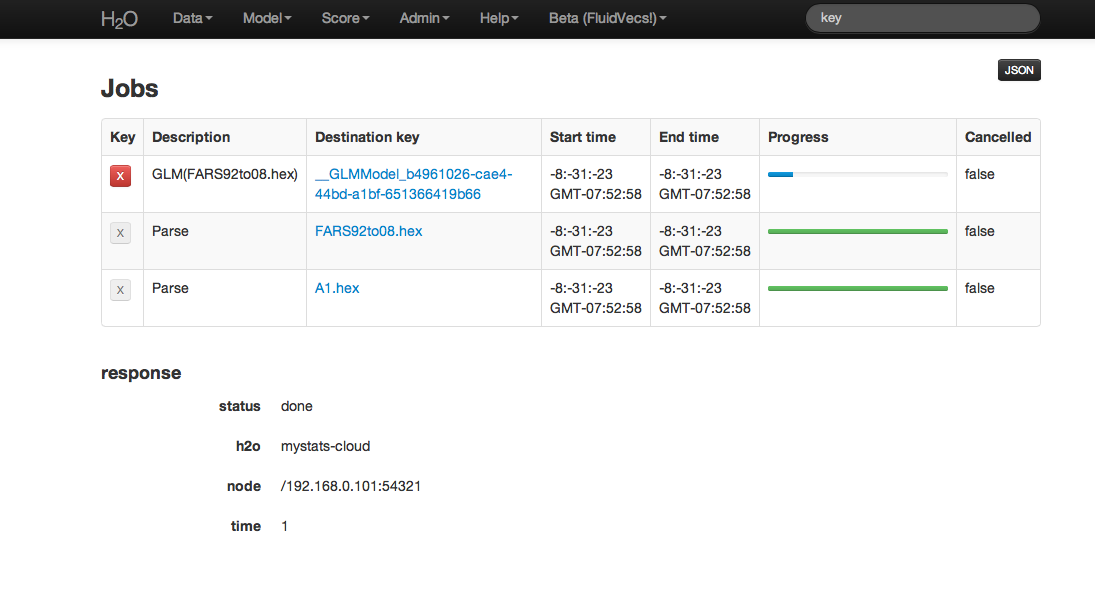
\includegraphics[height=5cm]{AdminJobs.jpg} \includegraphics[height=5cm]{DataViewAll.jpg}

\subsubsection{Variable importances} 

To enable the variable importances option, use the additional argument \texttt{importance=TRUE}. This displays the absolute and relative predictive strength of each feature in the prediction task. From R, access these strengths using the command \texttt{air.model@model\$varimp}. You can also view a visualization of the variable
importances on the web interface.

\subsubsection{Supported Output}

The following algorithm outputs are supported: 
\begin{itemize}
\item {\bf{Regression}}: Mean Squared Error (MSE), with an option to output variable importances or a Java POJO model
\item {\bf{Binary Classification}}: Confusion Matrix or Area Under Curve (AUC), with an option to output variable importances or a Java POJO model
\item {\bf{Classification}}: Confusion Matrix (with an option to output variable importances or a Java POJO model)
\end{itemize}

\subsubsection{Java model}  

To access Java (POJO) code to use to build the current model in Java, click the \textsc{Java model} button in the top right of a model summary page. If the model is small enough, the code for the model displays within the GUI; larger models can be inspected after downloading the model.
\\
\\
To download the model: 
\begin{enumerate}
\item Open the terminal window.
\item Create a directory where the model will be saved.
\item Set the new directory as the working directory.
\item Follow the curl and java compile commands displayed in the instructions at the top of the Java model.
\end{enumerate}

\subsection{Grid search for model comparison} 

To support grid search capabilities for model tuning,  specify sets of values for parameter arguments to tweak certain parameters and observe changes in model behavior. The following is an example of a grid search:

\begin{spverbatim}

air.grid <- h2o.gbm(y = "IsDepDelayed", x = myX, 
                   distribution="multinomial", 
                   data = air_train.hex, n.trees=c(5,10,15), 
                   interaction.depth=c(2,3,4), 
                   shrinkage=c(0.1,0.2))

\end{spverbatim}
\noindent
This example specifies three different tree numbers, three different tree sizes, and two different shrinkage values. This grid search model effectively trains eighteen different models over the possible combinations of these parameters. Of course, sets of other parameters can be specified for a larger space of models. This allows for more subtle insights in the model tuning and selection process, especially during inspection and comparison of the trained models after the grid search process is complete. To decide how and when to choose different parameter configurations in a grid search, refer to the beginning section for parameter descriptions and suggested values.

\begin{spverbatim}
# print out all prediction errors and run times of the models
air.grid
air.grid@model

# print out a *short* summary of each of the models (indexed by parameter)
air.grid@sumtable

# print out *full* summary of each of the models
all_params = lapply(air.grid@model, function(x) { x@model$params })
all_params

# access a particular parameter across all models
shrinkages = lapply(air.grid@model, function(x) { x@model$params$shrinkage })

shrinkages
\end{spverbatim}

\section{Conclusion}

Gradient boosted machines sequentially fit new models to provide a more accurate estimate of a response variable in supervised learning tasks such as regression and classification. Though notorious for being difficult to distribute and parallelize, H2O's GBM offers both features in its framework, along with a straightforward environment for model tuning and selection. 

\newpage

\section{References}

Click, Cliff and SriSatish Ambati. {\textbf{"Cliff Click Explains GBM at Netflix October 10 2013"}} \url{http://www.slideshare.net/0xdata/cliff-click-explains-gbm} SlideShare (2013).  
\\
\\
Dietterich, Thomas G, and Eun Bae Kong. {\textbf{“Machine Learning Bias, Statistical Bias, and Statistical Variance of Decision Tree Algorithms.”}} \url{http://www.iiia.csic.es/~vtorra/tr-bias.pdf} ML-95 255 (1995).
\\
\\
Elith, Jane, John R Leathwick, and Trevor Hastie. {\textbf{“A Working Guide to Boosted Regression Trees.”}} \url{http://onlinelibrary.wiley.com/doi/10.1111/j.1365-2656.2008.01390.x/abstract} Journal of Animal Ecology 77.4 (2008): 802-813
\\
\\
Friedman, Jerome H. {\textbf{“Greedy Function Approximation: A Gradient Boosting Machine.”}} \url{http://statweb.stanford.edu/~jhf/ftp/trebst.pdf} Annals of Statistics (2001): 1189-1232.
\\
\\
Friedman, Jerome, Trevor Hastie, Saharon Rosset, Robert Tibshirani, and Ji Zhu. {\textbf{“Discussion of Boosting Papers.”}}\url{http://web.stanford.edu/~hastie/Papers/boost_discussion.pdf} Ann. Statist 32 (2004): 102-107
\\
\\
Friedman, Jerome, Trevor Hastie, and Robert Tibshirani. {\textbf{``Additive Logistic Regression: A Statistical View of Boosting (With Discussion and a Rejoinder by the Authors).”}} \url{http://projecteuclid.org/DPubS?service=UI&version=1.0&verb=Display&handle=euclid.aos/1016218223} The Annals of Statistics 28.2 (2000): 337-407
\\
\\
Hastie, Trevor, Robert Tibshirani, and J Jerome H Friedman. {\textbf{The Elements of Statistical Learning}}  \url{http://statweb.stanford.edu/~tibs/ElemStatLearn/printings/ESLII_print10.pdf}. Vol.1. N.p., page 339: Springer New York, 2001. 
\\
\\




\end{document}
